%\documentclass[12pt,a4paper]{book}
%\usepackage[utf8]{inputenc}
%\usepackage[portuguese]{babel}
%\usepackage[T1]{fontenc}
%\usepackage{amsmath}
%\usepackage{amsfonts}
%\usepackage{amssymb}
%\usepackage{graphicx}
%\usepackage{lmodern}
%\usepackage[left=2cm,right=2cm,top=2cm,bottom=2cm]{geometry}
%\author{Rodrigo Câmara}
%\title{Questões e atividades de Cálculo Numérico}
%\makeindex
%\usepackage{amsthm}
%\theoremstyle{remark}
%\newtheorem{ex}{Questão}[chapter]
%\begin{document}
\section{Aritmética do ponto flutuante}
%\subsubsection{Exercícios}


\begin{ex}
Represente os seguintes números na base binária. Algum destes números não pode ser exatamente representável em uma máquina? 
\begin{multicols}{2}
\begin{enumerate}[label=\alph*)]
\item $(25)_{10}$
\item $(11)_{10}$
\item $(15)_{10}$
\item $(0.1875)_{10}$
\item $(25.75)_{10}$
\item $(0.6)_{10}$
%\item $\pi$
\item $\frac{3}{4}$
%\item $\frac{•}{•}$
\end{enumerate}
\end{multicols}
\begin{sol}
\begin{enumerate}[label=\alph*)]
\item $(11001)_2$
\item $(1011)_2$
\item $(1111)_2$
\item $(0.0011)_2$
\item $(11001.11)_2$
\item $(0.10011001100110011...)_2.$ A única forma de representar este número exatamente é utilizando \emph{infinitos} algarismos. Em um computador com um número \emph{finito} de algarismos, esse número não pode ser exatamente representado.
\end{enumerate}
\end{sol}
\end{ex}


\begin{ex}
Represente os seguintes números binários na forma decimal.
\begin{multicols}{2}
\begin{enumerate}[label=\alph*)]
\item $(1101)_2$
\item $(111)_2$
\item $(10)_2$
\item $(0.011)_2$
\item $(111.011)_2$
\end{enumerate}
\end{multicols}
\begin{sol}
\begin{enumerate}[label=\alph*)]
\item $(13)_{10}$
\item $(7)_{10}$
\item $(2)_{10}$
\item $(0.375)_{10}$
\item $(7.375)_{10}$
\end{enumerate}
\end{sol}
\end{ex}

\begin{ex}
Represente os seguintes números na forma normalizada:\label{ex.normalizada}
\begin{enumerate}[label=\alph*)]
\item $(100)_{10}$ 
\item $(0.0158)_{10}$
\item $(101)_2$
\end{enumerate}
\begin{sol}
\begin{enumerate}[label=\alph*)]
\item $0.1\times 10^3.$
\item $0.158\times 10^{-1}.$
\item $0.101\times 2^3.$
\end{enumerate}
\end{sol}
\end{ex}



\begin{ex}
Sobre o sistema de ponto flutuante normalizado $SPF (10,5,-15,20)$, que utiliza o arredondamento, faça o que é pedido:
\begin{enumerate}[label=\alph*)]
\item Como é representado o número 12.31419? \label{12}
\item Como é representado o número 250 001 000 000? \label{25}
\item Qual é o erro absoluto cometido por este sistema ao representar o número do item \ref{12}?
\item Qual é o erro absoluto cometido por este sistema ao representar o número do item \ref{25}?
\item Compare os dois erros absolutos. Que conclusões você pode tirar?
\item Como é representado o número $\frac{1234567}{100000000}$?\label{frac1}
\item Como é representado o número $\frac{1234567}{10}$?\label{frac2}
\item Qual é o erro absoluto cometido por este sistema ao representar o número do item \ref{frac1}? Idem para \ref{frac2}.
\item Compare os dois erros absolutos. Que conclusões você pode tirar?
\end{enumerate}
\begin{sol}
\begin{enumerate}[label=\alph*)]
\item $0.12314*10^2$ ou $0.12314E+2$.
\item $0.25000*10^{12}$ ou $0.25000E+12$.
\item Na notação usual, $0.00019$. Na notação de ponto flutuante normalizado, $0.19*10^3$.
\item $1000000$, ou $0.1*10^7$.
\end{enumerate}
\end{sol}
\end{ex}


\begin{ex}
Considere o sistema de ponto flutuante normalizado SPF (10,4,-1,2). Para este sistema,
\begin{enumerate}
[label=\alph*)]
\item Qual é o menor positivo exatamente representável?
\item Qual é o maior positivo exatamente representável?
\item Determine as regiões de \emph{overflow} e de \emph{underflow}.
\end{enumerate}
\begin{sol}
\begin{enumerate}
[label=\alph*)]
\item $0.1*10^{-1}$.
\item $0.9999*10^2$.
%\item \emph{Dica}: Não se esqueça que o primeiro dígito após o ponto deve ser diferente de zero. Não se esqueça também de contar os números negativos e o zero.
\item Região de \emph{overflow}: Todos os números maiores que $0.999*10^2$ e todos os números menores que $-0.999*10^2$. Região de \emph{underflow}: todos os números maiores que $-0.1*10^{-1}$ e menores que $0.1*10^{-1}$ (exceto o número zero).
\end{enumerate}
\end{sol}
\end{ex}




\begin{ex}
Considere uma máquina SPF(10,4,-16,16) que utiliza arredondamento. Calcule, de acordo com o modo de operação desta maquina, o resultado da expressão 
$$(((4+4)+4)+4)+56070.$$
Em seguida, considerando a mesma máquina, calcule 
$$(((56070+4)+4)+4)+4.$$
Que conclusões você tira?

	\begin{sol}
		\begin{align*}
		&(((4+4)+4)+4)+56070\\
		&=(((0.4*10^1+0.4*10^1)+4)+4)+56070\\
		&=((0.8*10^1+0.4*10^1)+4)+56070\\
		&=(0.12*10^2+0.4*10^1)+56070\\
		&=(0.12*10^2+0.04*10^2)+56070\\
		&=0.16*10^2+0.5607*10^5\\
		&=0.00016*10^5+0.5607*10^5\\
		&=0.56086*10^5\\
		&=0.5609*10^5.
		\end{align*}
		Agora, para os cálculos de $(((56070+4)+4)+4)+4$, observe que $56070+4$ é calculado como 
		\begin{align*}
		 &0.5607*10^5+0.4*10^1\\
		 &=0.5607*10^5+0.00004*10^5\\
		 &=0.56074*10^5\\
		 &=0.5607*10^5.
		\end{align*}Chegue à conclusão que a primeira expressão apresentada possui resultado diferente da segunda.
	\end{sol}

\end{ex}





\section{Problemas}
\begin{ex}
Quantos números podem ser exatamente representados em uma máquina $F(10,4,-1,2)$ que opera no sistema do ponto flutuante?
\end{ex}
\begin{ex}


\begin{quote}
 ``[...] Poucos dos números usados superam $10^{100}$, ou seja, o número $1$ seguido de cem zeros, que foi batizado \emph{googol} por um garoto de 9 anos, sobrinho do matemático americano Edward Kasner. Para se ter uma ideia, desde o \emph{Big Bang}, se passaram ``apenas'' $17\times 10^{39}$ ioctossegundos, a menor unidade de tempo observável. 

Apesar de ser um número absurdamente grande, contar até o \emph{googol} ou até 10 é parte do mesmo processo. Mas contar a totalidade dos números naturais é outro problema, pois é preciso compreender que muito grande e infinito são conceitos inteiramente diferentes. Pense um número muito, muito, muito, mas muito grande: esteja certo, ele não estará mais perto do infinito do que o 1. Mas essa é outra história...''\end{quote}

\begin{flushleft}
Adaptado da revista \emph{Superinteressante}, ``A magia dos grandes números'', disponível em \url{http://super.abril.com.br/ciencia/a-magia-dos-grandes-numeros/}, acesso em 20 de maio de 2017.
\end{flushleft}


É possível representar o número \emph{googol} em um computador que opera em aritmética de ponto flutuante $F(\beta,t,m,M)$? Caso seja possível, sugira os valores das configurações $\beta, t, m$ e $M$ de um computador que consegue representar perfeitamente este número. Caso não seja possível, explique o porquê.

\end{ex}


\begin{ex}
\begin{quote}

\emph{Pac-Man} é um jogo de \emph{videogame} lançado no Japão em 1980 para fliperamas. Foi um dos maiores sucessos da época e ainda hoje versões são lançadas em diversas plataformas modernas. 
O objetivo era controlar o personagem-título por um labirinto e devorar todas as pastilhas. No momento em que \emph{Pac-Man} consegue coletar todas elas, o jogador alcança a fase seguinte. 

\begin{figure}[h!b]
\center
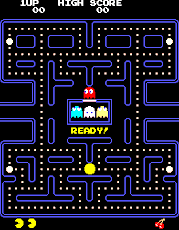
\includegraphics[width=0.23\linewidth]{pac}
\caption{O começo de uma fase de \emph{Pac-Man}}
\end{figure}

As fases são gradativamente mais rápidas e difíceis. No entanto, por melhor que seja o desafiante, ninguém consegue terminar o jogo: em uma dada fase, sempre acontece o ``\emph{killscreen bug}'' (o ``defeito da tela da morte''). O labirinto se deforma, letras invadem a tela e \emph{Pac-man} fica impedido de capturar todas as pastilhas da fase, tornando impossível a vitória (figura \ref{ch.erro.death}).

\begin{figure}[h!b]
\center
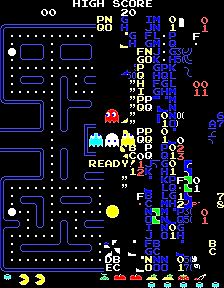
\includegraphics[width=0.23\linewidth]{death}
\caption{A fase com o “defeito da tela da morte”. Esta fase é não jogável.}\label{ch.erro.death}
\end{figure}


Como o defeito acontece? O número da fase na qual o jogador se encontra é registrado na memória em formato binário em um espaço de oito dígitos. O processador registra na memória a fase 1 como \texttt{00000001}; a fase 2 é registrada como \texttt{00000010}; a fase 3 é registrada como \texttt{00000011}; a fase 4 é \texttt{00000100}; a fase 5 é \texttt{00000101} e assim em diante.


O defeito acontece quando o processador tenta registrar um número maior que este espaço de memória de oito dígitos é capaz de armazenar.\end{quote}
Fonte: adaptado de \url{http://errors.wikia.com/wiki/Pac_Man_-_Infamous_Kill_Screen_Bug} 

Com base no texto acima, determine em qual fase acontece o defeito da tela da morte.
\end{ex}
\begin{ex}
Dentre os algoritmos de resolução de sistema linear temos o ``método de eliminação de Gauss''. Este algoritmo executa uma série de operações fundamentais com o intuito de simplificar um sistema de equações.

Digamos que, em um dado momento, o computador deva escolher entre exatamente uma dessas duas abordagens a se realizar:
\begin{itemize}
\item Multiplicar os números $d$, $e$ e $f$ por $\frac{1234567}{100000000}$ e somá-los com os números $a$, $b$ e $c$.
\item Realizar uma mudança de ordem nas linhas do sistema linear e, em seguida, multiplicar os números $d$, $e$ e $f$ por $\frac{1234567}{10}$ e somá-los com os números $g$, $h$ e $i$.
\end{itemize}
Supondo que ambas as abordagens \emph{teoricamente} produzem o mesmo resultado final e supondo que o computador opere em sistema de ponto flutuante com uma mantissa de cinco dígitos, existe alguma vantagem em uma abordagem em relação à outra? Explique.
\end{ex}





\begin{ex}
A tabela \ref{calculadora} lista as características de algumas calculadoras.

% Please add the following required packages to your document preamble:
% \usepackage{booktabs}
\begin{table}[h!b]
\centering
\caption{Configurações de algumas máquinas calculadoras.}
\label{calculadora}
\begin{tabular}{@{}llllll@{}}
\toprule
Fabricante         & Modelo           & Base, $\beta$ & Mantissa, $t$ & Expoente mín, $m$ & Expoente máx, $M$ \\ \midrule
\emph{CASIO}     & \emph{FX-82EX} & 10            & 10                       & -99                  & +99                  \\
\emph{HP}        & \emph{12c}     & 10            & 12                       & -99                  & +99                  \\
\emph{Microsoft} & \emph{Excel}   & 10            & 15                       & -307                 & 307                  \\
\emph{TexasInc}  & \emph{JJF85}   & 2             & 32                       & -64                  & 64                   \\ \bottomrule
\end{tabular}
\end{table}

Qual destas calculadoras consegue representar o maior número? E qual consegue representar o menor número positivo? Alguma dessas máquinas consegue representar exatamente o número \emph{googol}? Alguma dessas máquinas consegue representar exatamente o número $\pi$?
\end{ex}


\begin{ex}
Em 4 de junho de 1996, menos de um minuto após o lançamento, o foguete francês \emph{Ariane 501} se autodestruiu. Era o primeiro lançamento da série Ariane 5 e, logo em seguida, foi indicada pelo CNES (Centro Nacional de Estudos Espaciais) e pela ESA (Agência Espacial Europeia) uma comissão presidida pelo matemático francês Jacques-Louis Lions, do Colégio da França, para investigar o desastre.


Digamos que você faz parte dessa comissão e recebeu a tabela \ref{foguete} que indica os valores da função “alinhamento interno horizontal” (\emph{horizontal bias}¸ em inglês), $H(t)$, ao longo do tempo. Esta função indica para o foguete quanto combustível os propulsores horizontais devem queimar para alinhar o veículo. Os valores são calculados na central de comando, em uma máquina $F(10,12,-64,64)$, e enviados instantaneamente por rádio para o computador de controle do foguete, uma máquina $F(10,8,-16,16)$, ambas operando em sistemas de ponto flutuante.


% Please add the following required packages to your document preamble:
% \usepackage{booktabs}
\begin{table}[h!b]
\centering
\caption{Alinhamento interno horizontal do foguete, ao longo do tempo após o lançamento. Fonte \url{http://www.sbmac.org.br/bol/bol-2/artigos/ariane5.html}, acesso em 20 de maio de 2017.}
\label{foguete}
\begin{tabular}{@{}ll@{}}
\toprule
Tempo $t$, em segundos & Alinhamento interno horizontal, $H(t)$ \\ \midrule
0                      & 0                                      \\
5                      & 0.212542000000E4                             \\
10                     & 0.511252351123E10                      \\
15                     & 0.238114322137E11                      \\
20                     & 0.812001231123E11                      \\
25                     & 0.322016666667E12                      \\
30                     & 0.544406681249E15                      \\
35                     & 0.167731031031E20                      \\
40                     & 0.389310310310E34                      \\ \bottomrule
\end{tabular}
\end{table}


A partir da tabela \ref{foguete} você é capaz de determinar em qual momento (em segundos) aconteceu uma falha no \emph{software}? Qual falha aconteceu?

\end{ex}
